\documentclass[a4paper]{report}

%====================== PACKAGES ======================

%\usepackage[french]{babel}
\usepackage[utf8x]{inputenc}
%pour gérer les positionnement d'images
\usepackage{float}
\usepackage{amsmath}
\usepackage{graphicx}
\usepackage[colorinlistoftodos]{todonotes}
\usepackage{url}
%pour les informations sur un document compilé en PDF et les liens externes / internes
\usepackage{hyperref}
%pour la mise en page des tableaux
\usepackage{array}
\usepackage{tabularx}
%pour utiliser \floatbarrier
%\usepackage{placeins}
%\usepackage{floatrow}
%espacement entre les lignes
\usepackage{setspace}
%modifier la mise en page de l'abstract
\usepackage{abstract}
%police et mise en page (marges) du document
\usepackage[T1]{fontenc}
%\usepackage[top=2cm, bottom=2cm, left=2cm, right=2cm]{geometry}
%Pour les galerie d'images
\usepackage{subfig}
\usepackage{titlesec}
\titleformat{\chapter}[display]
  {\normalfont\huge\bfseries}{}{0pt}{\Huge}
\titlespacing*{\chapter}{0pt}{-20pt}{40pt}


%====================== INFORMATION ET REGLES ======================

%rajouter les numérotation pour les \paragraphe et \subparagraphe
\setcounter{secnumdepth}{4}
\setcounter{tocdepth}{4}

\hypersetup{							% Information sur le document
pdfauthor = {Premier Auteur,
			Deuxième Auteur,
			Troisième Auteur,
    		Quatrième Auteur},			% Auteurs
pdftitle = {Nom du Projet -
			Sujet du Projet},			% Titre du document
pdfsubject = {Mémoire de Projet},		% Sujet
pdfkeywords = {Tag1, Tag2, Tag3, ...},	% Mots-clefs
pdfstartview={FitH}}					% ajuste la page à la largueur de l'écran
%pdfcreator = {MikTeX},% Logiciel qui a crée le document
%pdfproducer = {}} % Société avec produit le logiciel

%======================== DEBUT DU DOCUMENT ========================

\begin{document}

%régler l'espacement entre les lignes
\newcommand{\HRule}{\rule{\linewidth}{0.5mm}}

%page de garde
\begin{titlepage}
\begin{center}

% Upper part of the page. The '~' is needed because only works if a paragraph has started.

\includegraphics[width=0.35\linewidth]{logo.jpg}~\\[1cm]

\textbf{\textsc{\LARGE Master 1 Computer Science}\\[1.5cm]}
\textsc{\Large }\\[0.5cm]

% Title
\HRule \\[0.4cm]

{\huge \bfseries Neural Networks Project\\
Football matches results predictor \\[0.4cm] }

\HRule \\[1.5cm]

% Author and supervisor
\begin{minipage}{0.4\textwidth}
\begin{flushleft} \large
\centering
\emph{Authors:}\\
\textsc{Yasmine Moussaoui}\\
\textsc{Dorian Fornali}\\
\textsc{Guillermo Wauquier}\\
\end{flushleft}
\end{minipage}





\vfill

% Bottom of the page
{\large \ November 2023}

\end{center}
\end{titlepage}







\tableofcontents
\thispagestyle{empty}
\setcounter{page}{0}
%ne pas numéroter le sommaire



%espacement entre les lignes d'un tableau
\renewcommand{\arraystretch}{1.5}

%====================== INCLUSION DES PARTIES ======================

~
\thispagestyle{empty}
%recommencer la numérotation des pages à "1"
\setcounter{page}{0}

\chapter{Project presentation}


\section{Presentation of the subject}

The subject of this project revolves around the creation of a sophisticated system dedicated to predicting sports outcomes. The main objective is to develop a robust tool capable of providing accurate predictions for various sports competitions. This system aims to leverage statistical data to generate victory probabilities, offering an insightful perspective on the expected performances of teams.

\section{Project aims}

\textbf{Overall Objective}

The fundamental objective of this project is the design and implementation of an advanced sports outcome prediction system. Efforts are concentrated on achieving two main goals:

\begin{quote}
\textbf{1) Modeling Victory Probabilities}

The first major objective is to develop a program capable, when presented with two teams (A and B), of generating a probability (p) representing the chance of victory for team A. This also involves determining the complementary probability of victory for team B (1\-p).



\textbf{2) Prediction of Finalists and Championship Results}

In a broader perspective, the project aims to process data from a specific championship to identify the finalist teams and predict the probability of victory for each finalist in the decisive match.
\end{quote}

\textbf{Methodological Approach}
To achieve these objectives, the methodological approach proposes the implementation of two distinct regressors. The first one uses a random forest (RF) model, while the second relies on a neural network (NN) with a multi-layer perceptron model.

\textbf{Parameter Optimization}
Emphasis is placed on the pursuit of excellence through the determination of an optimal set of parameters for each regressor. This critical step aims to ensure maximum performance when predicting probabilities.

\textbf{Model Evaluation and Selection}
The last step of the methodological approach involves evaluating the performance of the models. Tools such as the confusion matrix and various performance indicators derived from it will be used to choose the model that offers the most reliable and accurate results. In summary, the project combines an advanced algorithmic approach with methodological rigor to provide probable and informative sports predictions. These predictions apply to both specific match-ups and larger-scale competitions.


\chapter{Preparation of data}
\section{The "Cut"}
Firstly, let's take stock of the datasets at our disposal. We have four different datasets: results.csv (1872-present), goalscorers.csv (1916-present), shootouts.csv (1967-present), and rankings.csv (1992-present), along with fifa\_country\_list.csv.\\

When embarking on a project involving multiple datasets, it is crucial to start with proper data preparation. The key to any machine learning task lies in thorough data preparation.\\

In our case, the initial step involves a "cut" based on dates. The idea is straightforward: choose a date and retain all data prior to the selected date. Analyzing the project's datasets reveals a natural choice as we encounter four distinct dates: 1872, 1916, 1967, and 1992. These dates exhibit a considerable chronological gap.\\

Selecting the date for data filtering, however, proves to be more intricate. Several possibilities exist, and none are inherently incorrect. Beginning with the most obvious, considering 1872 is unnecessary. Football's origins at that time were more of a recreational activity for sailors than the internationally recognized professional sport we know today. Moreover, the involvement was primarily limited to British countries, making it incompatible with the project's goal of predicting a modern international football event.\\

Considering the first organized World Cup in 1930 could be a valid option. This aligns with the emergence of international football tournaments, including the World Cup, signifying a more developed global football scenario. However, this choice propels us too far ahead in time, where football significantly differed in terms of technology, rules, and World Cup format mutations.\\

The sentiment turns nostalgic when considering 1950 onwards. For many ardent football enthusiasts, sidestepping the football scene from 1950 onwards is inconceivable. The emergence of football stars such (Di Stefano,Pelé, Yashin, Eusebio), dynasties like Real Madrid and AC Milan, and prestigious trophies like the European Cup and Ballon d'Or make this period pivotal. Unfortunately, our model does not focus on this era.\\

After delineating reasons for not considering earlier dates that hold significance in football history, let's settle on the final date. We opted for a "cut" in 1996. This choice is influenced by the contemporary World Cup format with a total of 32 teams and the year 1996 marks the commencement of playoffs for the 1998 World Cup. This World Cup is of particular interest as it introduces the 32-team format for the first time. Mirroring what we aim to predict: the Qatar 2022 World Cup. By ending just before the Qatar World Cup, we ensure our predictions are unbiased.\\

Regulatory considerations play a role, too, as the rules in 1996 align closely with today's standards. Choosing an earlier date might introduce variations such as matches without offside rules, goalkeepers handling back passes from teammates'feet, and restrictions on substitutions.\\

To conclude this section, selecting 1996 ensures that all datasets are available, as they all provide data from 1992 onwards. This eliminates the need for additional internet searches to fill in missing data, especially relying on the intricate FIFA rankings, which would otherwise be challenging to recreate independently.\\
\newpage
\section{Fixes on the list of countries}

Choosing data from 1996 for analysis has significant advantages, especially regarding how countries are named. This approach avoids issues related to disappeared political entities, like the Soviet Union, and makes it easier to compare data among countries that have undergone changes in their names. By focusing on this period, we consider the disappearance of outdated entities, such as Yugoslavia, and the recognition of new states. This allows for analysis in a context where international relations have become more stable, while avoiding ambiguities related to naming countries during periods of political transition. Thus, analyzing data from 1996 provides a strong foundation for understanding the current political realities of countries while maintaining consistency in their national identification.\\

Our dataset could contain several countries with different or outdated nomenclatures; therefore, we had to organize the dataset.\\
\begin{figure}[h]
  \centering
  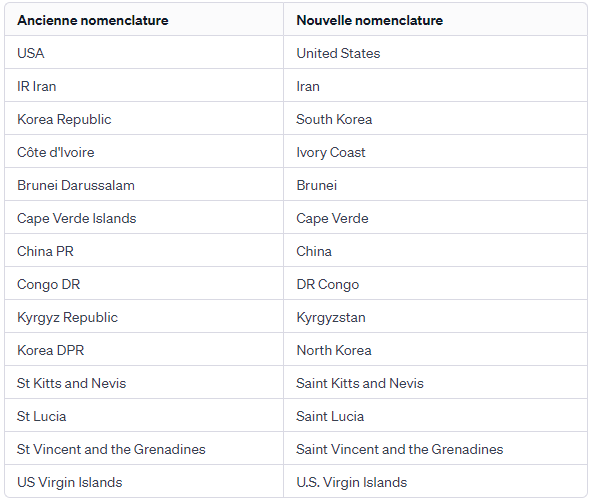
\includegraphics[width=0.8\linewidth]{countries.png}
  \caption{Mapping of Former and Updated Nomenclature in FIFA Rankings}
\end{figure}\\

\newpage
\section{Resampling}
Once the data has been filtered, we proceed to organize the new datasets. The initial step involves renaming "rank\_date" to "date" for uniform attributes. In this ongoing effort, we proceed to create a dataset named "daily\_ranking," which is essentially a version of the filtered rankings dataset but tailored for each unique date present in the filtered match results. This approach allows us to have a dataset that provides the ranking as of the date for each played match.
\section{Merging Data}
In this data merging step, the goal is to integrate information related to match results with daily rankings. Several operations are conducted for this purpose.
Firstly, a redundant column named 'country\_full' is dropped from the daily rankings DataFrame (daily\_ranking). This elimination is necessary to avoid conflicts during the subsequent merging of data. Additionally, the DataFrame's index is reset to convert the 'date' and 'country\_full' columns from index to regular columns, making it easier for future data manipulation.
The first merge is performed with the filtered match results DataFrame (results\_filtered). Data for home teams is merged using the 'home\_team' and 'date' columns from the results DataFrame and the 'country\_full' and 'date' columns from the modified daily rankings DataFrame. This operation employs the pd.merge method with the how='left' parameter, ensuring that all rows from the results DataFrame are included, while only the corresponding rows from the rankings DataFrame are added.
Post-merge, resulting columns are renamed to clearly indicate that they represent characteristics of the home team; for instance, 'rank' becomes 'home\_rank'. This step aims to enhance data comprehensibility and avoid potential confusion during subsequent analysis.
Next, a second merge is executed with the daily rankings DataFrame to incorporate features of the away teams. Similarly, the 'away\_team' and 'date' columns from the results DataFrame are matched with the 'country\_full' and 'date' columns from the rankings DataFrame, again using the pd.merge method with how='left'.
Once more, resulting columns are renamed, this time to indicate that they represent features of the away team; for example, 'rank' becomes 'away\_rank'.
In summary, this data merging step creates a new DataFrame called "rera" that seamlessly integrates relevant information for football match analysis, clearly distinguishing features of home and away teams. This process ensures data consistency and facilitates interpretation during subsequent analysis steps.



\chapter{Implementations of machine learning algorithms}

\section{Random Forest}
\subsection{Data Preparation}
In addition to all of the data manipulation and preparation we did to our datasets, we need, in fact, one last preparation phase in order to correctly train the model with our data. 

Since we work with a regressor random forest (and not a classifier), the model requires numerical data, which mean, for instance, the home\_team and away\_team features (=columns) need to be modified into numerical values.
To achieve this, we one-hot encoded all our categorical features.
One-hot encoding in machine learning is the conversion of categorical information into a format that may be fed into machine learning algorithms to improve prediction accuracy.


To achieve this, we one-hot encoded all our categorical features.
One-hot encoding in machine learning is the conversion of categorical information into a format that may be fed into machine learning algorithms to improve prediction accuracy.

What it does in practice is to "divide" a feature into n features, where n is the amount of distinct values the feature had.

For example, the following dataframe:
\begin{table}[h]
  \centering
  \begin{tabular}{|c|}
    \hline
    Country\\
    \hline
    France
     \\
    \hline
    England\\
    \hline
    Wales\\
    \hline
  \end{tabular}
  \label{tab:exemple}
\end{table}


Will be encoded into the following dataframe:\\
\begin{table}[h]
  \centering
  \begin{tabular}{|c|c|c|}
    \hline
    Country\_France & Country\_England & Country\_Wales \\
    \hline
    1 & 0 & 0 \\
    \hline
    0 & 1 & 0 \\
    \hline
    0 & 0 & 1 \\
    \hline
  \end{tabular}
  \label{tab:exemple}
\end{table}

\newpage
Using that method, we encoded every categorical features of our final dataset. 
One other preparation we could have done for the model is to normalize our numerical values, to ensure every feature has the same impact and "weight"
However, in the case of Random Forests, the nature of the algorithm, which builds decision trees based on feature splits, inherently handles varying scales without the need for explicit normalization.

We tested this property and found it was true.\\
\begin{figure}[h]
  \centering
  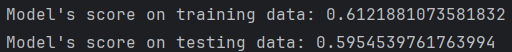
\includegraphics[width=0.8\linewidth]{withNormalization.png}
  \caption{Here the model's accuracy with the normalization}
\end{figure}

\begin{figure}[h]
  \centering
  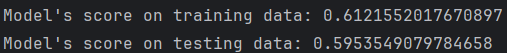
\includegraphics[width=0.8\linewidth]{withoutNormalization.png}
  \caption{Here the model's accuracy without the normalization}
\end{figure}

\subsection{Training and best parameters}
Our data is finally ready to be used by the random forest regressor.
As mentionned earlier, we used scikit learn's RandomForestRegressor class as our model.
The regressor variant allows us to target multiple features to predict in contrary to the classifier random forest.
We chose to predict the $home\_score$ and $away\_score$, the amount of goals the teams scored.
Scikitlearn also proposes the GridSearchCV class, a very powerful tool that will determine the best possible parameters configuration for the model.

Once created and set with the best parameters, we need to train the model with our dataset. 
It's our final step before being able to predict a match.

In order to train the model we must split our dataframe into the training samples and the testing samples.
We did that using the $test\_train\_split()$ function from scikitlearn model selection library.
We decided to take 70\% of the dataframe for training purpose and thus 30\% for testing.

For the training, scikitlearn proposes an already built-in function for the RandomForestRegressor class which is fit() that we used.
In fact, things are a bit different in the project because we train the GridSearchCV, and we extract our trained model from this object.

\begin{verbatim}
randomForestModel = RandomForestRegressor(random_state=1)
randomForestGridSearch = 
GridSearchCV(randomForestModel, params, cv=5, verbose=1, n_jobs=-1)
\end{verbatim}

\noindent Then we train the model
\begin{verbatim}
randomForestGridSearch.fit(X_train, y_train)
\end{verbatim}

\noindent We apply to our model the best parameters found by the grid search
\begin{verbatim}
randomForestModel = randomForestGridSearch.best_estimator_
\end{verbatim}


\subsection{Prediction}
To predict a match or a championship (see Championship part later) we need to give to our model an entry (a row) in the shape of what it has been trained on. Basically speaking, we give him as input a dataframe with a single row, without, obviously, the features to predict (the scores).
The input also needs to be encoded the exact same way the training set was.
In our code, the getMatchDataframe() does this job, with just the names of the playing countries and the city/country host of the match, we fetch all the remaining data to have our input.

For example we fetch the latest rank from the FIFA ranking dataset, the latest averageScore from $rera\_improved$ and so on ...
Also, the tournament in which the match takes place is always the FIFA World cup.
We also one hot encode the dataframe the same way it was done for the model training set

Finally, we use the predict() method of the model on that dataframe describing the match to predict the resulting scores.
We convert these scores into a probability of winning with an exponential fonction. The team with the highest probability wins. If the probabilites are near 50\%, we "simulate" a shootout. (See shoutouts part)

\subsection{Accuracy}
Our regressor random forest has an accuracy of near 60\% on the testing set, which is not very good.
Also, it appears that the model has a mean square error near 1, which is extremely high considering the predicted scores vary between 0.2 and 2.0.
Even although to us humans, the results are pretty decent, in a mathematical point of view the model is pretty unusable.
\subsection{Difficulties encountered for the Random Forest}
During the implementation of the Random Forest regressor, we met two main issues:
 \begin{itemize}
    \item[-] Understanding how to prepare the data for training the model was the hardest and longest part, which made us rollback 2 days of work to restart on a good base.
    \item[-] The most complex one: the model seems to very largely advantage the $home\_team$ even if the match is played at a neutral location.

\end{itemize}
	In others words, France - England would output France as the winner, and England - France would output England even if the matches were played in Australia for instance.
	Except when the strength difference was enough to outpower that disadvantage, the team on the left was always winning.
	To counter this bias we decided to predict two times the match, once A vs B and a second time B vs A. We then chose as the winner the winner of the match which had the biggest score difference, we thought it was a good solution.
\newpage
\section{Neural Network regressed}
\section{Comparison}
\section{Championship}
One goal of this project was to predict a championship.
The championship is in the shape of a .csv file containing the team groups.

First comes the group phase, where each team in a group plays a match against every other country in the same group. A win results in obtaining 3 points, and a draw 1 point for both team, there are no shootouts in this phase.

Once all the matches are played, the two teams with the highest points of their team go to the knockout phase. 
The knockout phase, the looser is eliminated and the winner goes to the next match, until one team is left, the champion.
In this phase, if the model outputs a very similar probability of winning for both teams, we simulate a shootout between the two teams. (See shootouts part)

Example of a championship predicted by the regressor random forest -
Here we tried to predict the 2022 world cup
\begin{figure}[h]
  \centering
  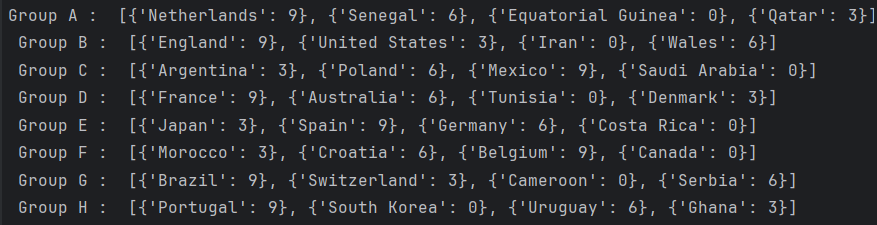
\includegraphics[width=0.8\linewidth]{cdmGroupPhase.png}
  \caption{Here are the group phase results with each team points}
\end{figure}

We can observe two main "anomalies" in these results, the Argentina is eliminated without reaching the knockout phase, and the Mexico won all its matches.
It is very hard to predict a World Cup since pretty much everything can happen (see for example Morocco's performance in World cup 2022), so calling it an anomaly isn't very pertinent.

\begin{figure}[h]
  \centering
  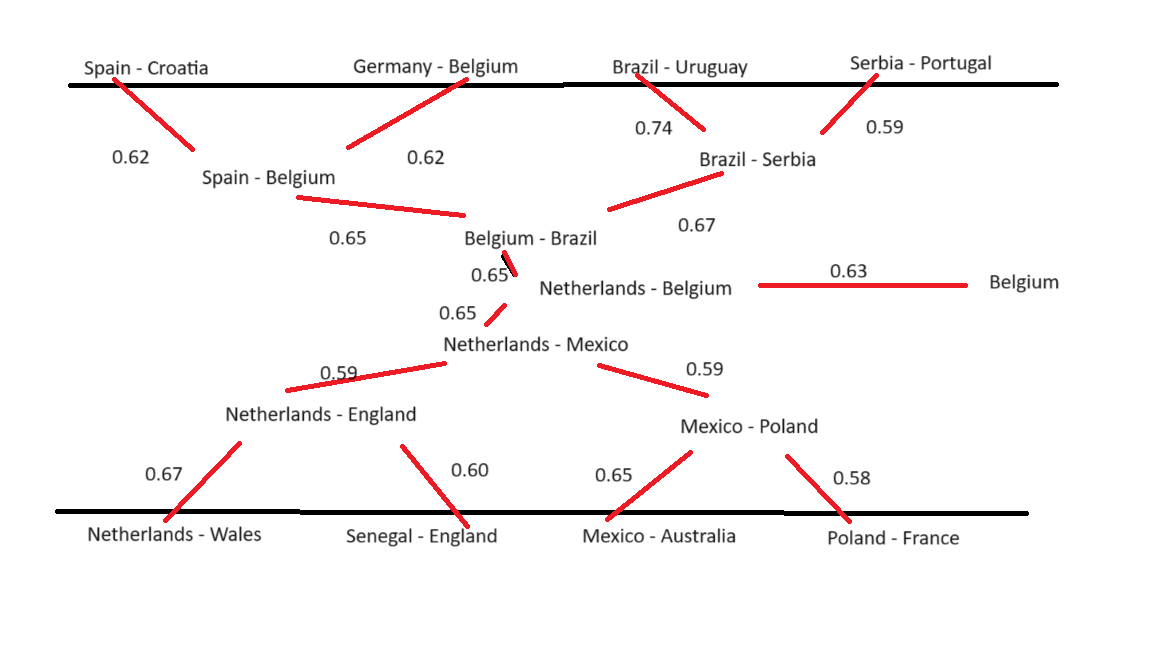
\includegraphics[width=0.8\linewidth]{championshipPaint.png}
  \caption{here is the knockout phase with the probabilities of win for every match}
\end{figure}

\newpage
\section{Shootouts}

%tableau à taille fixée sur certaines colonnes (param sur la ligne \begin{tabularx}, voir wiki pour plus d'info sur la syntaxe
\begin{figure}[!h]
\begin{center}
\begin{tabularx}{17cm}{|c|p{6cm}|X|}
  \hline
  Priorité & Nom & Raison\\
  \hline
  1 & Tache 1 & Doit être vérifié en premier car sinon [...] \tabularnewline
  2 & Tache 2 & On doit pouvoir [...] \tabularnewline
  3 & Tache 3 & Comme les principales fonctionnalités permettant de tester sont opérationnelles, nous pouvons passer à cette tâche. \tabularnewline
  4 & Tache 4 & Parce que [...] \tabularnewline
  5 & Tache 5 & La tache 5 fait partie des principales [...]. \tabularnewline
  6 & Tache 6 & Dernière fonctionnalité essentielle à mettre en place. \tabularnewline
  7 & Tache 7 & Non-essentiel, mais apporterait un plus au projet. \tabularnewline
  8 & Tache 8 & Non-essentiel, mais apporterait un plus au projet. \tabularnewline
  \hline
\end{tabularx}
\end{center}
\caption{Tableau récapitulatif des tâches}
\end{figure}

\chapter{Conclusion}
Our exploration into machine learning applications for football match prediction led us through crucial decisions in data preparation and the implementation of various algorithms. The choice to cut the data in 1996 proved essential, mitigating challenges related to changing political entities and ensuring consistent nomenclature. Structuring the dataset to accommodate country name changes was a pivotal organizational step, laying the groundwork for meaningful analysis and model implementation.\\


The implementation of a regression random forest showed successes and challenges, with 60\% accuracy, biases favoring the home team, and limitations in handling certain scenarios. Championship predictions illustrated the algorithm's ability to simulate complex football dynamics.\\


The implementation of a regression neural network revealed the model's sensitivity to dataset size, with the simpler random forest outperforming the neural network. Correlation analysis provided insights into feature relevance, contributing to a more informed data preparation approach.\\


In conclusion, the two models present divergent results. The random forest offers consistent but less precise predictions, while the neural network generates more chaotic predictions. The random forest appears better suited to this type of dataset, but the addition of additional datasets, such as team composition or medical conditions, could enhance overall prediction accuracy. This journey underscores the need for a balanced approach between model sophistication, data context, and adaptability to the inherent unpredictability of ever-evolving football.


%Ne pas numéroter cette partie
\part*{Annexes}
%Rajouter la ligne "Annexes" dans le sommaire
\addcontentsline{toc}{part}{Annexes}

\chapter*{Annexe 1}




%récupérer les citation avec "/footnotemark"
\nocite{*}

%choix du style de la biblio
\bibliographystyle{plain}
%inclusion de la biblio
\bibliography{bibliographie.bib}
%voir wiki pour plus d'information sur la syntaxe des entrées d'une bibliographie

\end{document}